%!TEX root = ../thesis.tex
%*******************************************************************************
%****************************** Seventh Chapter **********************************
%*******************************************************************************

\chapter{Homeostasis Optimisation}

\section[Optimisation Motivations]{Optimisation Motivations}

This section introduces the motivation for optimization in neuromorphic computing systems, with a specific focus on the challenges posed by analogue hardware implementations. Unlike digital systems, analogue memristive devices are inherently imprecise and subject to a variety of non-idealities, such as stuck states, limited dynamic range, and line resistance. The section outlines how these physical constraints impact computation accuracy and how algorithmic or circuit-level techniques can be leveraged to mitigate their effects.

\subsection[Analogue Hardware Challenges]{Analogue Hardware Challenges}

\noindent Novel computer hardware solutions that employ analogue devices still exhibit limited precision and unreliability. However, both physical and algorithmic techniques can be employed to mitigate these issues. In contrast to digital technology, the analogue approach inherently involves a degree of imprecision. \\

\noindent Analogue devices, such as RRAM, are susceptible to a number of issues, including stuck states, device-to-device variability and I-V nonlinearity. However, the development of advanced fabrication methods and circuit-level optimisations has enabled the mitigation of some of these non-idealities, while algorithmic techniques have also been shown to be effective in reducing their impact.\\

\noindent In contrast to the digital paradigm, where a multitude of physical imperfections are effectively concealed within a bit representation (either '1' or '0'), analogue electronics is confronted with significant challenges due to the intrinsic imprecision associated with non-discrete systems. Even with a minimal amount of non-idealities, it is challenging to encode information with perfect precision using an exact conductance value.\\

\noindent However, non-idealities do exist and can result in significant deviations from ideal behaviour. These include the device becoming stuck in certain conductance states, undergoing changes in conductance over time, showing non-linear current-voltage characteristics, or displaying non-linear conductance modulation in response to voltage stimuli. \\

\noindent It could be argued that analogue computing's more fundamental challenge lies in its reduced precision compared to digital computing, especially when digital systems utilise 16 or more bits of representation. While these issues may be grounds for disqualification in many applications, this may not be the case for machine learning applications, which often employ reduced precision computing, even within digital systems. \\

\noindent In general, machine learning models demonstrate a degree of robustness to minor alterations, such as the presence of noise \cite{cheney2017robustness}. In the event of significant deviations from ideal conditions, hardware imperfections may result in a decline in accuracy. However, this does not necessarily render the system inoperable. It is, therefore, crucial to comprehend the impact of non-idealities and to ascertain how they can be effectively mitigated. \\

\noindent In the context of linear algebra applications, a proportional relationship between voltage and current (i.e. Ohmic behaviour) is the preferred option. This is due to the fact that Ohm's law is employed in the implementation of multiplication, as previously discussed. Nevertheless, exceptions to this linear relationship do arise, particularly in the case of high-resistance devices \cite{mehonic2017intrinsic}. \\

\noindent A number of approaches exist at the device and circuit level that facilitate the resolution or even circumvention of the issue of nonlinearity. During the fabrication of RRAM devices, the adoption of a hot-forming step can result in the generation of more linear characteristics \cite{sung2018effect}. \\

\noindent In the case of individual device programming, the adoption of a transistor-to-resistor ratio (1T1R) architecture can facilitate the precise tuning of memristor conductance, despite the presence of any I-V nonlinearities \cite{li2018analogue}. Alternatively, a charge-based accumulation approach can be employed, wherein a constant voltage is applied, but the input is encoded into pulse width \cite{amirsoleimani2020memory}. This eliminates the dependence on the shape of the I-V curve. \\

\noindent It is possible that some memristive devices may become fixed in a specific conductance state. This phenomenon has been observed following processes such as electroforming, as well as after several successful programming cycles \cite{joksas2022nonideality}. In general, the greater the discrepancy between the intended and actual conductance, the greater the potential for adverse effects. Therefore, it is of paramount importance to identify methods for the prevention or mitigation of faulty devices.\\

\noindent The overall effect of a device becoming stuck is contingent upon the behaviour of other devices, and thus this phenomenon can be employed to mitigate the negative effects. To illustrate, if a device becomes stuck, its negative effect may be counteracted by adjusting the conductance of another device in the differential pair \cite{liu2017rescuing}. On occasion, such an adjustment may occur accidentally, whereby both devices in a differential pair become stuck simultaneously.\\

\noindent As an alternative, if faulty devices can be identified prior to programming, more sophisticated mapping strategies can be employed. The most significant weights can be mapped onto crossbar rows and columns with the lowest incidence of stuck devices \cite{gaol2021reliable}. The most significant terms refer to the weights that could have the greatest impact on accuracy. One way to identify such weights is to calculate of sensitivity $\Delta w_{i,j} := - \eta \frac{\partial E}{\partial \Delta w_{i,j}}$, for each weight $w_{i,j}$, where \textit{E} is the back-propagated loss at the current neuron and $\eta$ is the learning rate.\\

\noindent The term 'limited dynamic range nonideality' is used to describe a situation whereby the $\frac{G_{on}}{G_{off}}$ ratio is relatively small, which can ultimately result in a reduction in effective precision. In the context of other non-idealities, such as device variability, limited dynamic range can result in a reduction in the number of distinguishable states that are available. \\

\noindent If each state is associated with a certain amount of absolute variability, it is evident that a larger dynamic range is preferable, as it allows for a more effective differentiation between those states that are less distinct. The impact of the dynamic range is highly dependent on the specific application. Should one desire to utilise analogue arrays for the storage of digital information, an enhanced dynamic range will facilitate a greater precision in the number of equivalent bits.\\

\noindent Nevertheless, when considering the acceleration of linear algebra operations (and, by extension, machine learning), such comparisons cannot be made with the same degree of ease. As these hardware accelerators are based on analogue computation, the concept of 'bits' – although potentially useful – does not apply directly. In analogue contexts, an error is defined as any deviation from the intended value. The magnitude of the error is the key factor in determining the severity of the mistake. \\

\noindent In the context of inference applications, a large dynamic range is not a crucial factor. If a naive mapping scheme is employed whereby the value of a weight is represented using a single conductance value, then the inaccuracies produced by this imperfect mapping can be addressed with a $\frac{G_{on}}{G_{off}}$ ratio of as low as 3 \cite{mehonic2019simulation}. In other contexts, the impact of limited dynamic range cannot be evaluated without first understanding the nature of other non-idealities, namely the deviations they cause.\\

\noindent Line resistance represents a non-ideality that arises from the presence of non-zero interconnect resistances in crossbar arrays. In the event of its presence, this results in discrepancies from the ideal computation of vector-matrix products. While the impact on accuracy can be significant, there are both physical and algorithmic techniques that can be employed to mitigate it. \\

\noindent One of the most straightforward methods for mitigating the impact of line resistance is to enhance the ratio between the resistance of the devices and the resistance of the interconnecting wires. As resistance is inversely proportional to the cross-sectional area of the wire, one method of reducing interconnect resistance is to increase the width of the wires \cite{li2017three}.\\

\noindent However, this can be challenging in dense arrays, and an alternative approach is to use more conductive materials, for example, $2nm$ platinum nanofins \cite{pi2019memristor}. Another approach is to increase the resistance of the crossbar devices, although this can sometimes result in less stable device behaviour. \\

\noindent At the circuit level, a variety of techniques may be employed which utilise the systematic properties of line resistance in different ways. For instance, a technique designated as double biasing can facilitate a more symmetrical distribution of electric potentials within crossbar arrays, thereby attenuating the impact of line resistance effects \cite{hu2016dot}. As the size of the crossbar array increases, voltage drops tend to accumulate. \\

\noindent Therefore, splitting up the array into smaller units \cite{xia2016technological}, or even organising them in three-dimensional structures \cite{xia2019memristive} can help to mitigate this issue. In considering the specific applications for which crossbar arrays are to be employed, algorithms may be deployed to ascertain optimal mappings from software parameters to physical quantities, such as voltage and conductance.  A nonlinear mapping from weights to conductances can be employed to counteract the detrimental effects of line resistance. \\

\noindent Alternatively, sensitivity analysis can identify the weights that are most sensitive, and thus map them closest to the applied voltages, where their contribution would be disturbed the least \cite{agrawal2019x}. In the specific context of supervised learning, input intensities may be predicted, and the inputs with the highest expected intensity (as well as the corresponding weights) can be mapped closest to the outputs in order to minimise the negative effects of line resistance. \\

\noindent When training networks directly on crossbar arrays, i.e. in situ, linear adjustments of conductance are the preferred approach \cite{burr2015experimental}. In order to ensure a linear response, the system must be modified physically. Some previous studies have proposed adjusting the device structure \cite{woo2016improved}, typically by introducing additional layers \cite{wu2018methodology}. An alternative approach is combining memristive devices with CMOS transistors, which help to improve the linearity \cite{ambrogio2018equivalent}.\\

\noindent Random telegraph noise (RTN) is defined as the occurrence of unpredictable switching between two or more discrete voltage levels in electronic devices \cite{puglisi2016guidelines}. This phenomenon is frequently observed in memristors. RTN is more commonly experienced in devices with higher resistance, which can impede the use of such devices for reducing power consumption or mitigating the effects of line resistance. To circumvent RTN or at least mitigate its effects, it is necessary to modify the fabrication process. For instance, some studies have demonstrated that non-filamentary devices can assist in reducing this type of noise \cite{chai2018impact}. \\

\noindent Once the specific application where memristive crossbars will be employed is identified—for instance, classification using neural networks, a pertinent metric such as accuracy, may be optimised instead of attempting to address individual non-idealities. This methodology is more technology-agnostic, as the nature of non-idealities frequently differs between technologies. However, approaches that optimise the metrics pertinent to the application tend to be algorithmic and, thus, more readily transferable.\\

\noindent In the field of machine learning, averaging approaches have the potential to enhance the accuracy and robustness of models, particularly in situations where the memristive implementation is susceptible to non-idealities. One strategy is to utilise multiple networks in parallel and compute their average outputs. Additionally, stability over time can be a crucial consideration, as certain non-idealities, such as RTN, are stochastic in nature. By averaging over time, the effects of these non-idealities can be mitigated \cite{wan2020voltage}.\\

\noindent The statistical approaches employed in modern machine learning are based on the minimisation of deviations from ideal behaviour in the training data. This can be extended to incorporate the non-ideal effects of the hardware on which the model will be implemented. In some instances, this can be achieved by introducing non-ideality-agnostic noise during training in order to enhance the robustness of the networks \cite{ye2023improving}. Alternatively, noise can be designed to reflect the nature of the non-idealities, thereby enabling the model to adapt more effectively to the various shortcomings of the hardware \cite{huang2021method}.

\subsection[Optimisation Approaches]{Optimisation Approaches}

Spike-based optimisation techniques seek to minimise the overall error of a network by optimising the times of individual neuron spikes. As the time at which a neuron spikes is a continuous value, continuous optimisation methods can be employed. However, the problem remains highly non-linear due to the potential for a small change in the input to a neuron (and thus a small change to the neuron's input weights) to push the neuron over its firing threshold, eliciting a spike and drastically changing the neuron's output \cite{gutig2014spike}. \\

\noindent The initial algorithm to perform supervised deep learning by optimising spike times was SpikeProp \cite{bohte2002error}. This algorithm makes the simplifying assumption that each neuron will fire at most one spike during the spiking interval. In the event that multiple spikes are fired, only the first is optimised. Additionally, each connection is composed of numerous synaptic terminals, each with a distinct synaptic delay and connection weight. \\

\noindent The authors demonstrate that their algorithm can solve the XOR problem and performs comparably to backpropagation, which has been optimized both with gradient descent (GD) and Levenberg-Marquardt (LM), on a number of small datasets (the largest of which has 36 input dimensions, six output classes, and 4,435 training examples). \\

\noindent The single-spike optimisation procedure and multiple connection weights per synapse have presented significant challenges in expanding this work to larger datasets. Another work \cite{mckennoch2006fast} presented two methods to improve the rate of convergence of SpikeProp; however, the applications remain limited to small datasets. \\

\noindent Another publication put forth an alternative to the SpikeProp algorithm \cite{mostafa2017supervised}, which was designed with the specific intention of accommodating non-leaky integrate-and-fire neurons. The proposed method relaxes the restriction that a connection must be composed of many different discrete-delay elements, and instead employs a more standard network architecture, with one exponential-synapse connection between each pair of neurons. The networks were trained with both one and two hidden layers, achieving 2.45\% and 2.86\% accuracy on the MNIST dataset, respectively. \\

\noindent One challenge encountered by the author was that the dropout technique, the most commonly employed regularisation method, was ineffective in the network under consideration. This was because it frequently resulted in the complete cessation of neuronal firing. In the absence of an efficacious alternative regularisation method, the networks exhibited considerable generalisation errors, the training error for both networks was almost zero.\\

\noindent While earlier algorithms focused on optimising the initial spike of each neuron, another relaxed this constraint by employing a genetic algorithm to enhance multiple spikes from each neuron \cite{stromatias2015supervised}. However, they limited their demonstration to relatively modest models comprising fewer than 10 hidden neurons. Genetic algorithms frequently encounter challenges in scaling to problems with numerous parameters, raising concerns about the scalability of this algorithm to datasets such as MNIST or CIFAR-10.\\

\noindent In a similar vein, another publication \cite{lee2016training} also optimise over multiple spikes per neuron. The authors disregard the spiking discontinuity that occurs during backpropagation, instead treating the output of a neuron as a linear function of its inputs, which have been filtered by the membrane of the neuron in question. This enables the network to be run in spiking neurons during training, while still performing backpropagation without concern for discontinuities. \\

\noindent Furthermore, the refractory period of the neurons is disregarded, as it is deemed to be relatively brief in comparison to the time interval between spikes, and therefore has a minimal impact on firing rates. In order to enhance the performance of the network, lateral inhibition components are introduced; however, only the first-order derivatives caused by these connections are optimised. \\

\noindent Notwithstanding these simplifications, their method is still capable of learning appropriately on the MNIST task, achieving 1.30\% error using standard SGD and 1.23\% error using an ADAM optimiser. While it remains to be seen whether this method can generalise to larger datasets in a tractable way, it introduces a number of new ideas for training spiking networks that will hopefully be improved upon by future work. \\

\noindent A different study introduce a novel method for making the spiking process continuous \cite{huh2018gradient}. They introduce a gating function, \textit{g(V)}, of the membrane voltage, \textit{V}, that is greater than zero for voltages approaching the firing threshold and zero otherwise, with unit integral. The region where $g(V) > 0$ is referred to as the active zone. \\

\noindent In contrast to the conventional approach, whereby efferent synapses receive a current $\delta (t - t_k)$ upon the neuron crossing the firing threshold at time $t_k$, this method allows synapses to continuously receive current based on $g(V)\frac{dV}{dt}$. In the event that the voltage is situated outside the active zone, this term is rendered zero due to the fact that \textit{g(V)} is equal to zero. \\

\noindent Conversely, should the voltage traverse the active zone (and thus the neuron spike), the integral of this term is equal to one. Ultimately, if the voltage enters the active zone but does not exceed the upper threshold (i.e., the firing threshold), the integral of the term will be a positive number between zero and one (this is analogous to a partial spike). \\

\noindent This induced synaptic current is nearly identical to the traditional spiking current $\delta (t - t_k)$ in the extreme cases (i.e., when the neuron is silent or firing at a relatively high rate), but continuous in the intermediate region. The authors may then achieve a gradient through the network at any given point in time by employing backpropagation, and optimise the entire network by utilising backpropagation through time.\\

\noindent The results presented focus on tasks that require a dynamic, temporal representation, such as predictive coding. This represents a distinct focus in comparison to the majority of other spike-based methods, which tend to prioritise static tasks (such as object classification). Consequently, a direct comparison is challenging. \\

\noindent As a consequence of the method rendering the neural nonlinearity differentiable, a multitude of distinct neuron models may be employed. The present paper utilises non-leaky integrate-and-fire and quadratic integrate-and-fire models, with a plethora of alternative models being equally compatible. \\

\noindent This, in conjunction with the capacity to optimise recurrent spiking networks effectively, renders this a potentially potent methodology for dynamic spiking networks. In the context of networks specialising in static tasks, it is postulated that the necessity for this method to optimise over potentially lengthy time series for each input stimulus would render it unsuitable for training large object classification networks. \\

\noindent To date, spike-based optimisation methods have yet to be applied to larger, deeper architectures such as convolutional neural networks (CNNs). This has precluded the implementation of spike-based training on any datasets that are either larger or more challenging than the MNIST dataset. \\

\noindent One of the challenges lies in the computational requirements of spike-based optimisation methods, which necessitate more computational resources than rate-based methods. This is due to the dynamic nature of the network and the iterative simulation required for each stimulus presentation. \\

\noindent The majority of existing software has been designed for static artificial neural networks (ANNs), and extending it to spiking networks is a complex undertaking. Consequently, researchers have employed rate-based optimisation methods to address larger datasets with spiking networks, which will be discussed next. \\

\noindent Rate-based optimisation methods operate under the simplifying assumption that all neurons are engaged in rate coding. Consequently, these methods are indifferent to the times of individual spikes, focusing instead on the number of spikes occurring within a given time period. \\

\noindent In the majority of cases, these types of methods utilise this simplifying assumption to replace the spiking neural process with a continuous-valued rate approximation. In the case of derivative-based methods, this rate approximation is then differentiated. Derivative-free methods, in contrast, circumvent the necessity of taking the derivative of this rate approximation, instead opting for an optimisation method such as Contrastive Divergence that does not require it. \\

\noindent Finally, function approximation methods approach the problem from a different angle. Rather than assuming a network of spiking neurons and attempting to identify rate approximations to these spiking neurons, they select an arbitrary nonlinearity for training the network, and then employ spiking neurons to approximate this nonlinearity.


\section[Homeostasis Regularization]{Homeostasis Regularization}

This section introduces homeostasis as a biologically inspired mechanism for regularization in SNNs. By dynamically adjusting synaptic strength based on neuronal firing activity, homeostasis stabilizes learning and mitigates the impact of faulty or overactive devices. The section explores how this mechanism can be modeled mathematically and implemented in hardware to improve robustness and energy efficiency.

\subsection{Programming Variabilities}

One of the most common non-idealities observed in memristive devices is the phenomenon of devices becoming stuck. This topic was previously explored in depth in the preceding chapter. In this chapter, a similar model is employed, in which devices may become stuck at $G_{off}$ or $G_{on}$. For both types of simulations, a range of probability were used, indicating that any individual may become stuck in that state. Although this is a simple model, it is not data-specific, and thus could be combined with the nonidealities that were modelled using experimental data, specifically $SiO_x$ nonlinearities.\\

\noindent A more realistic probabilistic model for describing stuck device behaviour in crossbar array can be introduced. This is achieved by randomly drawing from a sample of all memristors and setting the conductance to the closest achievable state. Although this method is relatively robust given the high number of devices, it is discrete in nature and therefore more difficult to apply during SNN training, where gradients need to be computed. \\

\noindent Furthermore, the method is limited in data in certain conductance regions, which may result in training that fits the weights to the behaviour of a single instance of a crossbar array. Consequently, a more continuous approach to picking the states at which the devices may get stuck in was adopted.\\

\noindent It is possible to display previously encountered data; in this case, all potentiation and depression cycles are shown for some of the devices. The majority of memristors are capable of achieving a high conductance range, with only a small proportion exhibiting limited conductance or remaining in a fixed state. In this chapter, the simulations were conducted with $G_{off}$ and $G_{on}$ defined as the median of minimum and maximum conductances, respectively. \\

\noindent Any device whose maximum range (i.e., the difference between the highest and lowest conductances achieved) was less than half the median range (Gon - Goff) was classified as stuck. A further simplifying assumption was made that any such device would be treated as fully stuck. This overestimates the effect of the variability because in reality some of the 'stuck' devices may still be tweaked, albeit within a narrower range.\\

\noindent The challenge in constructing a probabilistic model in this case is the generation of a probability density function (PDF) that accurately describes the conductance values at which devices may become stuck. The selection of devices that may become stuck is a relatively straightforward process. \\

\noindent These devices can be chosen randomly, with the proportion of devices that fit the previously defined criteria for stuck behaviour being the determining factor. For instance, 10\% of the devices may be deemed to exhibit the necessary characteristics. However, the conversion of the discrete mean conductance values of these devices into a probability distribution that can be applied to a wider range of situations represents a more challenging aspect of this process.\\

\noindent In order to produce a probabilistic model, it was decided that kernel density estimation (KDE) would be employed. KDE is a method of producing a probability density function (PDF) given a sequence of randomly distributed variables. Each point is usually approximated with a random distribution, which are then summed together. \\

\noindent As these distributions are typically identical, the only choices that have to be made are the type of distributions to be used, or the width of those distributions, which is more commonly referred to as "bandwidth" \cite{turlach1993bandwidth} in the context of KDE. In this chapter, it was decided to employ truncated normal distributions, truncated at zero to circumvent the issue of negative conductance. \\

\noindent The underlying normal distributions were set to have a mean equal to the mean conductance of faulty devices, with the objective of estimating the standard deviation of the underlying distributions. In order to achieve this, Scott's rule \cite{scott2015multivariate} was utilised. As a consequence of the clipping of conductance values below zero, a bias is introduced, whereby the probability density is underestimated in the vicinity of the boundary, even if the PDF is re-scaled after truncation \cite{silverman2018density}. \\

\noindent To address this issue, a reflection method can be employed. Rather than performing re-normalisation, a second distribution was introduced, representing the reflection of the original normal distribution around zero. The negative part of this distribution was then clipped \cite{jones1993simple}. This approach ensures that the two truncated PDFs sum to one, while providing a more reliable estimate of the probability density near zero.\\

\noindent Furthermore, device-to-device (D2D) variability, which arises from inaccuracies during device programming, was also taken into account. As discussed in the preceding chapter, during the mapping of weights onto conductances, one may ultimately arrive at values that differ from the desired outcome. \\

\noindent Lognormal distribution is a commonly utilized approach to model these discrepancies. For instance, it has been demonstrated that resistance deviations adhere to this trend, with the relative (and consequently, the absolute) magnitude of the deviations being more pronounced in the high-resistance state (HRS) compared to the low-resistance state (LRS).\\

\noindent When weights \textit{W} are related to conductances \textit{G} monotonically (linearly in this case), regularization can influence both weights and conductances, providing a high-level tool for controlling power consumption. It has been proposed that the \textit{L1} sparsification regularizer \cite{han2015learning} should be employed, as it can both enhance training (e.g., by preventing overfitting) and promote lower conductance values. Instead of manually adjusting the mapping scheme, the network designer may prioritize low power consumption to varying degrees, for example, by adjusting the regularization factor in \textit{L1} regularization, which is incorporated into the conventional hyperparameter tuning process \cite{feurer2019hyperparameter} typically performed before SNN deployment.\\

\noindent Other recent studies have explored strategies to mitigate memristor non-idealities in SNNs \cite{morshed2023choose}. Advanced STDP implementations improve robustness through adaptive learning rates and probabilistic weight updates \cite{burr2017neuromorphic, pehle2022brainscales}. Hybrid analogue-digital designs improve consistency of weight storage \cite{friedmann2016demonstrating}. A promising approach exploits the subthreshold conduction regime, where low-power current transients encode precise temporal information \cite{mannion2023unipolar}, benefiting spike-based tasks such as neuromorphic vision \cite{mannion2020memristor}. This behaviour could improve the biological fidelity of learning mechanisms such as eligibility traces and homeostasis \cite{demiraug2021pcm, john2022reconfigurable}. In addition, homeostasis-driven dropout dynamically modulates synaptic conductance to prevent overfitting and stabilise learning \cite{vu2024spiking}. This section investigates subthreshold silicon oxide memristors in SNNs and proposes an adaptive dropout strategy for neuromorphic computing.\\

\begin{figure*}[!t]
    \centerline{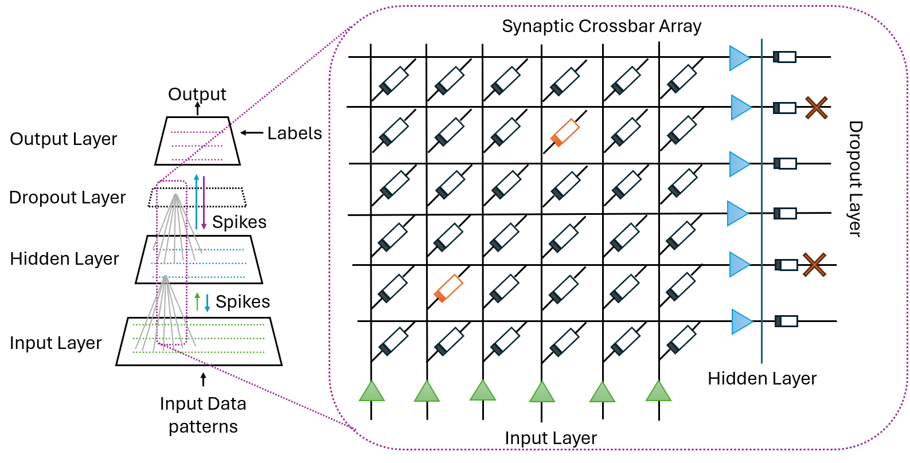
\includegraphics[width=0.95\textwidth]{Chapter7/Figs/a.png}}
    \caption[Proposed Neuromorphic architecture with homeostasis dropout]{Proposed Neuromorphic architecture with homeostasis dropout. A fully connected spiking neural network featuring input, hidden, dropout and output layers of spiking neurons, with synaptic connections illustrated for one neuron in the input and hidden layers. A portion of the neural network implemented with an RRAM crossbar memory array and neuron columns and rows, incorporating a homeostasis dropout layer for broken or overactive devices (red).}
    \label{fig:7a}
\end{figure*}
    

\noindent The described homeostasis mechanism can be applied as a dropout regularization layer in spiking neural networks (SNNs) \cite{stoffel2024spiking}. The synapse's conductance adjusts according to the firing frequency of the presynaptic neuron by utilising a non-monotonic response to the input firing rate. At lower firing rates, the conductance is higher, while at higher frequencies, it decreases, promoting synaptic depression. This behavior enables the system to suppress the influence of overactive or faulty neurons by adapting the conductance individually for each synapse. The advantage of this approach lies in its simplicity, as it does not require the presynaptic neuron to produce pulses of opposite polarity nor access to the postsynaptic side, thereby simplifying circuit design and enhancing regularization in SNNs. \\

\noindent In order to implement dropout regularization in spiking neural networks (SNNs), a homeostasis mechanism is employed that adjusts the synaptic conductance based on the input neuron’s firing rate \cite{kim2021spiking}. The synaptic conductance \( G \) is modeled as a function of the firing rate \( r_{\text{in}} \) of the presynaptic neuron. Specifically, the steady-state conductance \( G_{\text{steady}} \) is defined as a non-monotonic function of \( r_{\text{in}} \), where the conductance increases at lower firing rates and decreases when the firing rate surpasses a threshold, thereby inducing synaptic depression. The functional relationship between the firing rate and synaptic conductance is given by the following:
\begin{equation}
G_{\text{steady}} = \frac{G_{\text{max}}}{1 + \left(\frac{r_{\text{in}}}{r_{\text{threshold}}}\right)^n} \label{eq:7.1}
\end{equation}


\noindent Here, \( G_{\text{max}} \) represents the maximum conductance, \( r_{\text{threshold}} \) is the firing rate at which depression begins, and \( n \) controls the sharpness of the transition. This model allows for the suppression of synapses connected to neurons exhibiting high-frequency activity, effectively implementing a form of dropout. The output current \( I_{\text{out}} \) from the synapse is then determined by the product of the synaptic conductance \( G_{\text{steady}} \) and the input voltage \( V_{\text{in}} \):
\begin{equation}
I_{\text{out}} = G_{\text{steady}} \cdot V_{\text{in}} \label{eq:7.2}
\end{equation}

\noindent This dynamic adjustment of conductance provides a mechanism for selectively reducing the influence of overactive neurons during training, akin to traditional dropout in conventional neural networks. By modulating synaptic conductance based on firing rates, this approach ensures that only relevant connections are active, improving the network's robustness and preventing overfitting. \\

\begin{figure*}[!t]
    \centerline{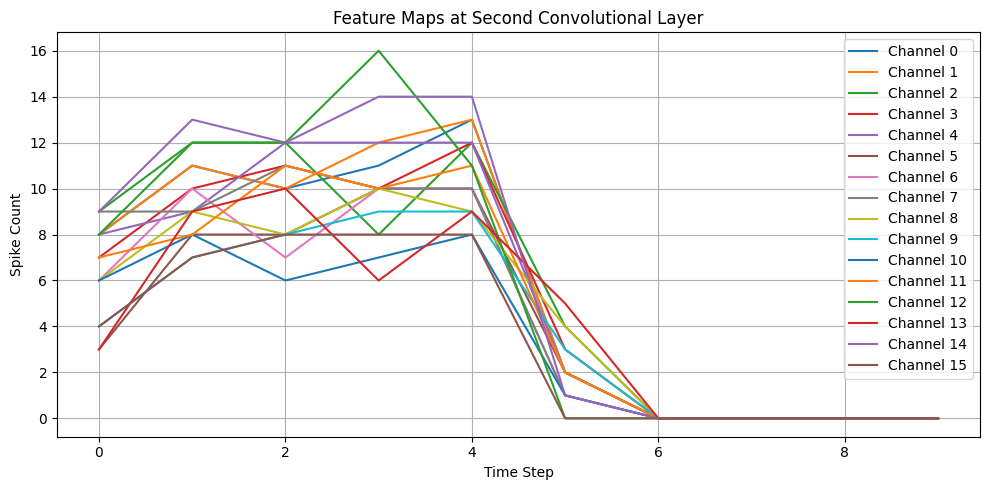
\includegraphics[width=0.8\textwidth]{Chapter7/Figs/b.png}}
    \caption[Feature maps at the second convolutional layer.]{Feature maps at the second convolutional layer. The plot demonstrates the suppression of simulated hyperactive neurons in a memristive spiking neural network for a convolutional layer with 16 hidden channels, at a threshold of 5 time steps.}
    \label{fig:7b}
\end{figure*}

\noindent The homeostasis-dropout method utilizes the time-step mechanism in SNN by focusing on the outputs from a window of the latest selected time steps instead of averaging across all steps. By dynamically adjusting synaptic conductance based on firing rates, this approach identifies a time-local window of significant activity, enabling selective suppression of overactive neurons. This not only reduces computational costs by avoiding redundant evaluations but also enhances robustness and prevents overfitting by emphasizing the most relevant temporal features during training and inference.

\subsection{Dropout Improvement}


\noindent A two-layer memristive Spiking Neural Network (MSNN) was designed to evaluate its performance on the MNIST dataset, which was converted into spike trains.The network, with a batch size of 64, was trained on 60,000 samples and tested on 10,000. The network contains 100 hidden neurons with Leaky Integrate-and-Fire (LIF) activation and a 10-neuron output layer.Synaptic weights were initialised randomly and updated during training over 1 epoch, with a learning rate of 5e-4 and 50 steps per epoch for 20 epochs.A homeostasis mechanism temporarily disables neurons with excessive spike activity to maintain stable dynamics.\\ 

\noindent The enhanced model, Memristive Convolutional Spiking Neural Network (MCSNN), incorporates convolutional layers to extract more complex features. The MCSNN includes a first convolutional layer with 12 filters using a 5x5 kernel, followed by 2x2 pooling, and a second convolutional layer with 64 filters, also followed by 2x2 pooling. The final layer is a memristive fully connected layer with 10 output neurons.The MCSNN, like the MSNN, uses LIF activation and a digital implementation for compatibility with existing hardware.\\

\noindent Both models are trained with the same hyperparameters, and the cross-entropy loss function from PyTorch is used for training, automatically managing softmax activation of the output layer.The architecture also incorporates kernel density estimation (KDE) to simulate the probabilistic nature of memristor failures and device-to-device variations, and most importantly to observe homeostasis.\\

\begin{figure*}[!t]
    \centerline{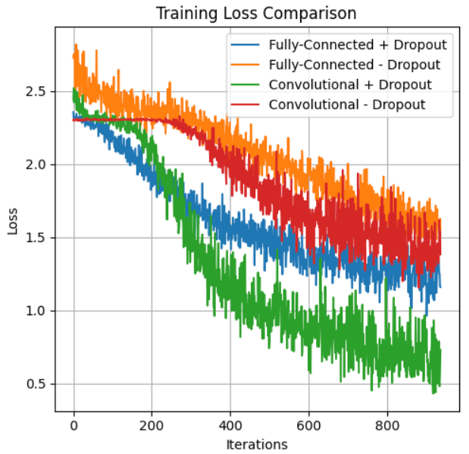
\includegraphics[width=0.6\textwidth]{Chapter7/Figs/c.png}}
    \caption[Training loss curve for standard and memristive schemes when exposed to I-V nonlinearities]{Training loss curve for standard and memristive schemes when exposed to I-V nonlinearities. The loss curves are noisy due to the tracking of losses at every iteration, rather than averaging across multiple iterations.}
    \label{fig:7c}
\end{figure*}


\noindent The training results demonstrate the impact of homeostasis dropout under simulated memristor failures and device-to-device variations at 50\%. Training curves for the MNIST dataset (Fig.\ref{fig:7c}) illustrate the differences between models with and without dropout, with dropout-enhanced models achieving lower loss and outperforming models with simulated faulty devices, particularly in convolutional architectures. \\

\begin{figure*}[!t]
    \centerline{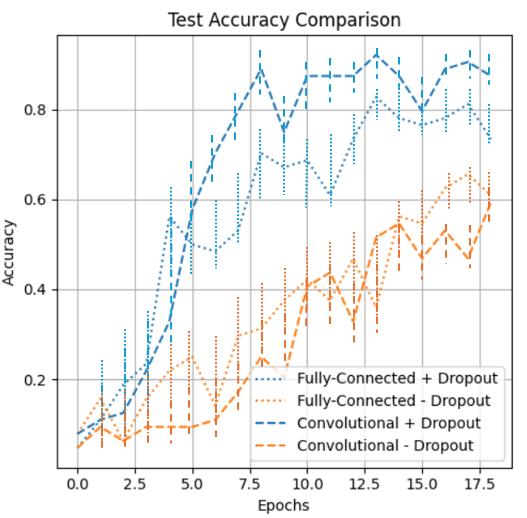
\includegraphics[width=0.6\textwidth]{Chapter7/Figs/d.png}}
    \caption[Training accuracy curve for standard and memristive schemes when exposed to I-V nonlinearities]{Training accuracy curve for standard and memristive schemes when exposed to I-V nonlinearities. Comparison of different spiking neural network performance when implemented with I-V nonlinearities from a single training run.}
    \label{fig:7d}
\end{figure*}
    
\noindent Figure\ref{fig:7d} compares accuracies between SNN and CSNN models, with dropout-improved versions reaching 80-90\%, while models with overactive neurons stabilized at ~60\% after 20 epochs. To address the high variability of non-idealities, which were nondeterministic, five networks were trained for each separate configuration. The results are summarised in table \ref{table:7a}, which demonstrates the efficacy of dropout in mitigating variability and improving performance in SNNs. \\

\begin{table}[!t]
    \caption{Model Accuracy for different SNN configurations}
    \begin{center}
    \begin{tabular}{|c|c|c|}
    \hline
    Model Accuracy  & Homeostasis Dropout & Memristor Failures \\ \hline
    Fully-Connected & $83.37 \pm 3.41 \%$  & $61.54 \pm 4.86 \%$ \\ \hline
    Convolutional   & $91.14 \pm 2.36 \%$  & $65.21 \pm 5.19 \%$  \\ \hline
    \end{tabular}
    \label{table:7a}
    \end{center}
    \vspace*{-\baselineskip}
\end{table}


\noindent In SNN, the membrane potential determines the likelihood of spike emission. During training, the membrane potential is used to compute the loss by comparing the output spike train to the target. When the potential exceeds a threshold, a spike is generated, signaling the neuron to "fire". This is where the homeostasis mechanism applies, as it adjusts synaptic conductance based on the input firing rates. Since the homeostasis regulates spike dynamics instead of direct membrane potential calculation, it acts as a regularization mechanism, modulating synaptic activity. The non-monotonic conductance model mimics biological synaptic plasticity, balancing excitation and inhibition. This balance improves generalization by preventing overfitting, akin to traditional dropout in deep learning.\\

\noindent The subthreshold regime enhances energy efficiency by minimizing current draw, a crucial advantage for edge AI applications. However, its inherently narrow resistance range compromises resilience to voltage noise, increasing susceptibility to errors in large-scale implementations. In complex SNNs, accumulated variations from device non-idealities—such as stochastic switching and drift—can compound over time, degrading overall performance. \\

\begin{figure*}[!t]
    \centerline{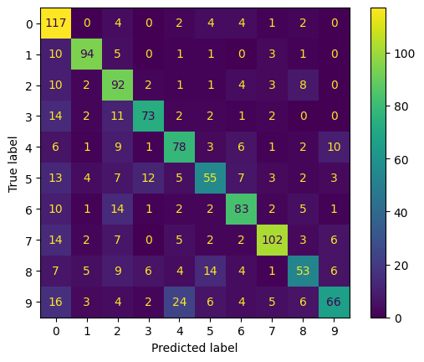
\includegraphics[width=0.6\textwidth]{Chapter7/Figs/e.png}}
    \caption[Confusion matrix of convolutional homeostasis model.]{Confusion matrix for successfully learned MNIST features during validation of convolutional homeostasis model.}
    \label{fig:7e}
\end{figure*}

\noindent While compensation strategies like adaptive learning rules or redundancy help mitigate these effects, they introduce computational overhead that may hinder real-time processing. Furthermore, fabrication inconsistencies can lead to deviations not fully captured by existing models, necessitating further optimization. Achieving both efficiency and robustness remains critical for scaling memristor-based neuromorphic systems in practical deployments.

\section[Biosignal Processing]{Biosignal Processing}

This section explores the applicability of memristive SNNs in processing time-sensitive biological signals such as EEG and MEG. Leveraging the event-driven and energy-efficient characteristics of SNNs, the section discusses their integration with convolutional layers to process spatiotemporal features in biosignals. The advantages over traditional deep learning models are highlighted, particularly in real-time, edge-computing applications.

\subsection{Architecture Adaptation}

Biosignals such as Electroencephalogram (EEG) and magnetoencephalogram (MEG) signals carry complex, time-sensitive information about brain activity that traditional deep learning models often struggle to efficiently process. Spiking Neural Networks (SNNs), which encode data as discrete spikes, more closely resemble biological neural signaling and offer significant improvements in temporal precision and energy efficiency compared to conventional Artificial Neural Networks (ANNs).\\

\noindent When augmented with convolutional layers, Convolutional SNNs (CSNNs) harness the spatial-temporal feature extraction power of CNNs while maintaining the sparse and event-driven nature of spiking neurons. CSNNs can achieve >99\% accuracy in detecting anticipatory EEG potentials—signaling user intent—in real-time applications such as braking systems, outperforming standard CNNs and other architectures \cite{lutes2024convolutional}. Similarly CSNNs applied to EEG-based stress detection achieve 98.7\% accuracy, highlighting their robustness and energy-conscious performance \cite{Joshi2025-sa}. \\

\noindent Nevertheless, the implementation of large-scale, low-power SNNs on conventional hardware remains challenging. Memristive hardware has been identified as a potentially effective solution to this issue. The deployment of synaptic weights directly within the fabric of crossbar arrays enables efficient native in-memory computing. This combination of temporal fidelity through event-driven spiking dynamics, energy-efficient spatial feature extraction via convolutional architectures, and ultra-low-power, compact hardware realisation enabled by in-memory memristive technologies represents a significant advance in the field.\\

\noindent Collectively, these characteristics position memristive CSNNs as a potent solution for real-time, on-device biosignal applications, rendering them particularly well-suited for portable, battery-sensitive settings such as brain-computer interfaces, stress monitoring, and ambulatory neurological diagnostics.\\

\noindent To begin, EEG and MEG obtained from the MGH/HMS/MIT Athinoula A. Martinos Center for Biomedical Imaging using the Neuromag Vectorview system \cite{Gramfort2020-jm}. EEG recordings were obtained through a 60-channel electrode cap that was synchronized with the MEG system, allowing for simultaneous acquisition of electrophysiological signals from the scalp and magnetic field changes associated with neuronal activity. \\

% \noindent Structural MRI data for the subject were collected separately using a Siemens 1.5 T Sonata scanner with a magnetization-prepared rapid acquisition gradient-echo (MPRAGE) sequence, providing high-resolution anatomical images suitable for source localization and co-registration with EEG/MEG data.\\

\noindent During the experiment, subjects were exposed to a sequence of stimuli consisting of visual and auditory inputs. Specifically, checkerboard patterns were displayed in either the left or right visual field, and tones were delivered to either the left or right ear. These stimuli were presented at regular intervals of 750 ms. At unpredictable intervals, a smiley face appeared at the center of the screen, serving as a visual target to which the participant was instructed to respond by pressing a button with the right index finger as quickly as possible.\\

\noindent Each type of stimulus and response was encoded using specific trigger codes: auditory left (LA = 1), auditory right (RA = 2), visual left (LV = 3), visual right (RV = 4), smiley face (smiley = 5), and button press (button = 32). These trigger events were embedded into the EEG/MEG recordings to enable precise epoching and event-related analysis.\\

\noindent In order to preprocess this data using the MNE-Python library \cite{gramfort2014mne}, the raw EEG and MEG recordings are first loaded, then event triggers are extracted, which identifies the timestamps and codes of all stimulus and response events. The data is then subjected to band-pass filtering, a process that serves to remove noise and artefacts. The selection of appropriate low and high cut-off frequencies is typically undertaken at this stage (e.g., 1–40 Hz). Epochs are created around each event, specifying the time window relative to each stimulus onset (e.g., -0.2 to 0.5 seconds).\\

\noindent Baseline correction is typically implemented within a pre-stimulus window (e.g., -0.2 to 0 s) with the objective of reducing drift and enhancing signal clarity. Furthermore, artifact rejection methods such as Independent Component Analysis (ICA) were employed to remove eye-blink or muscle-related artifacts. \\

\noindent The preprocessed epochs can subsequently be utilised for further analysis, including event-related potential (ERP) averaging, time-frequency decomposition, and source localisation. All signals were z-score normalized per channel and resampled to a uniform temporal resolution. The preprocessed EEG segments were formatted as tensors of shape $[B,C,T,N]$, where $B=64$ denotes batch size, $C=1$ is the input channel, $T=376$ is timepoints, and $N=71$ is the number of EEG channels.\\

\noindent The proposed hybrid Convolutional Spiking Neural Network (CSNN) architecture integrates the spatial pattern recognition strengths of Convolutional Neural Networks (CNNs) with the temporal sensitivity of Spiking Neural Networks (SNNs). In contrast to conventional recurrent models such as BiLSTMs \cite{malviya2022novel}, the CSNN does not incorporate sequential memory components. Instead, it employs event-driven temporal processing via spiking neurons, thereby reducing inference latency and energy consumption while maintaining temporal modelling fidelity. \\

\noindent The model commences with phase-based or latency-based spike encoding of electroencephalographic (EEG) signals. Specifically, a threshold-based latency encoding scheme was employed, whereby spike latency is inversely proportional to signal amplitude within each designated window. The encoded spike trains are then passed to the first convolutional layer, which applies 2D spatial filters over the spatiotemporal EEG input. The output of each convolutional layer is governed by the spiking dynamics:
\begin{equation} h_{ij}^{l} = \sigma \left( \sum _{k} w_{k}^{l} \cdot x_{(i+k)(j+k)} + b^{l} \right) \label{eq:7.3}
\end{equation}

\noindent Where $h_{ij}^{l}$ is the output at position $(i,j)$, $ w_{k}^{l}$ is the filter weight, and $\sigma$ is the activation function modeled for spiking dynamics \cite{tavanaei2019deep}. Each convolutional stage is followed by Leaky Integrate-and-Fire (LIF) spiking neurons, including optional homeostatic dropout layers, which regularize firing activity based on dynamic conductance principles inspired by oxide-based memristors.\\

\noindent In order to capture hierarchical representations, a stack of multiple convolution + LIF blocks with max pooling is employed \cite{shrestha2018slayer}. The final spiking representation is flattened and subsequently passed to the fully connected layers. This is followed by another layer of LIF neuron output layers. The temporal dynamics are addressed through the utilisation of spiking recurrence across timesteps, employing a backpropagation-through-time (BPTT) approach with surrogate gradients. This training strategy ensures differentiability despite the binary nature of spike outputs by approximating the Heaviside step function using smooth activations.

\subsection{Edge Evaluation}

The MCSNN was trained using cross-entropy loss computed on the spike rate of the output neurons, averaged over time. Optimization was performed using the Adam optimizer with weight decay, and training was conducted over 20-50 epochs depending on convergence behavior. The model was evaluated using accuracy and loss on a held-out test set. To visualize learned representations, feature maps from the output LIF layer were extracted and projected into lower dimensions using PCA, t-SNE, and UMAP embeddings.\\

\noindent These methods were used to embed high-dimensional spiking feature maps into two-dimensional spaces, enabling visualization of class-wise separation and classification decision boundaries using a logistic regression classifier. Performance was assessed through decision region plots and confusion matrices, each comprising four stimulus classes: auditory/left, auditory/right, visual/left, and visual/right.\\

\noindent The comparison of dimensionality reduction techniques—PCA, t-SNE, and UMAP—reveals distinct strengths and limitations when applied to feature representations extracted from the Memristive Convolutional Spiking Neural Network (MCSNN) trained on EEG data. Principal Component Analysis (PCA), a linear technique, provides a global view of the data structure and preserves large-variance directions but struggles to separate non-linearly distributed classes in this context. In contrast, t-distributed Stochastic Neighbor Embedding (t-SNE) excels at uncovering local structure, forming well-separated clusters that correspond closely to the EEG task classes; however, it may distort global relationships and is sensitive to hyperparameters like perplexity. \\

\noindent Uniform Manifold Approximation and Projection (UMAP) offers a balance between local and global preservation, maintaining neighborhood integrity while forming more compact and interpretable clusters than PCA, and with greater computational efficiency and scalability than t-SNE. The confusion matrices and decision boundaries further highlight that both t-SNE and UMAP result in higher class separability compared to PCA, with UMAP offering more stable performance across different runs. Overall, UMAP appears to be the most effective technique for visualizing and classifying nonlinearly embedded EEG features in the spiking domain.\\

\begin{figure}[htbp!]
    \centerline{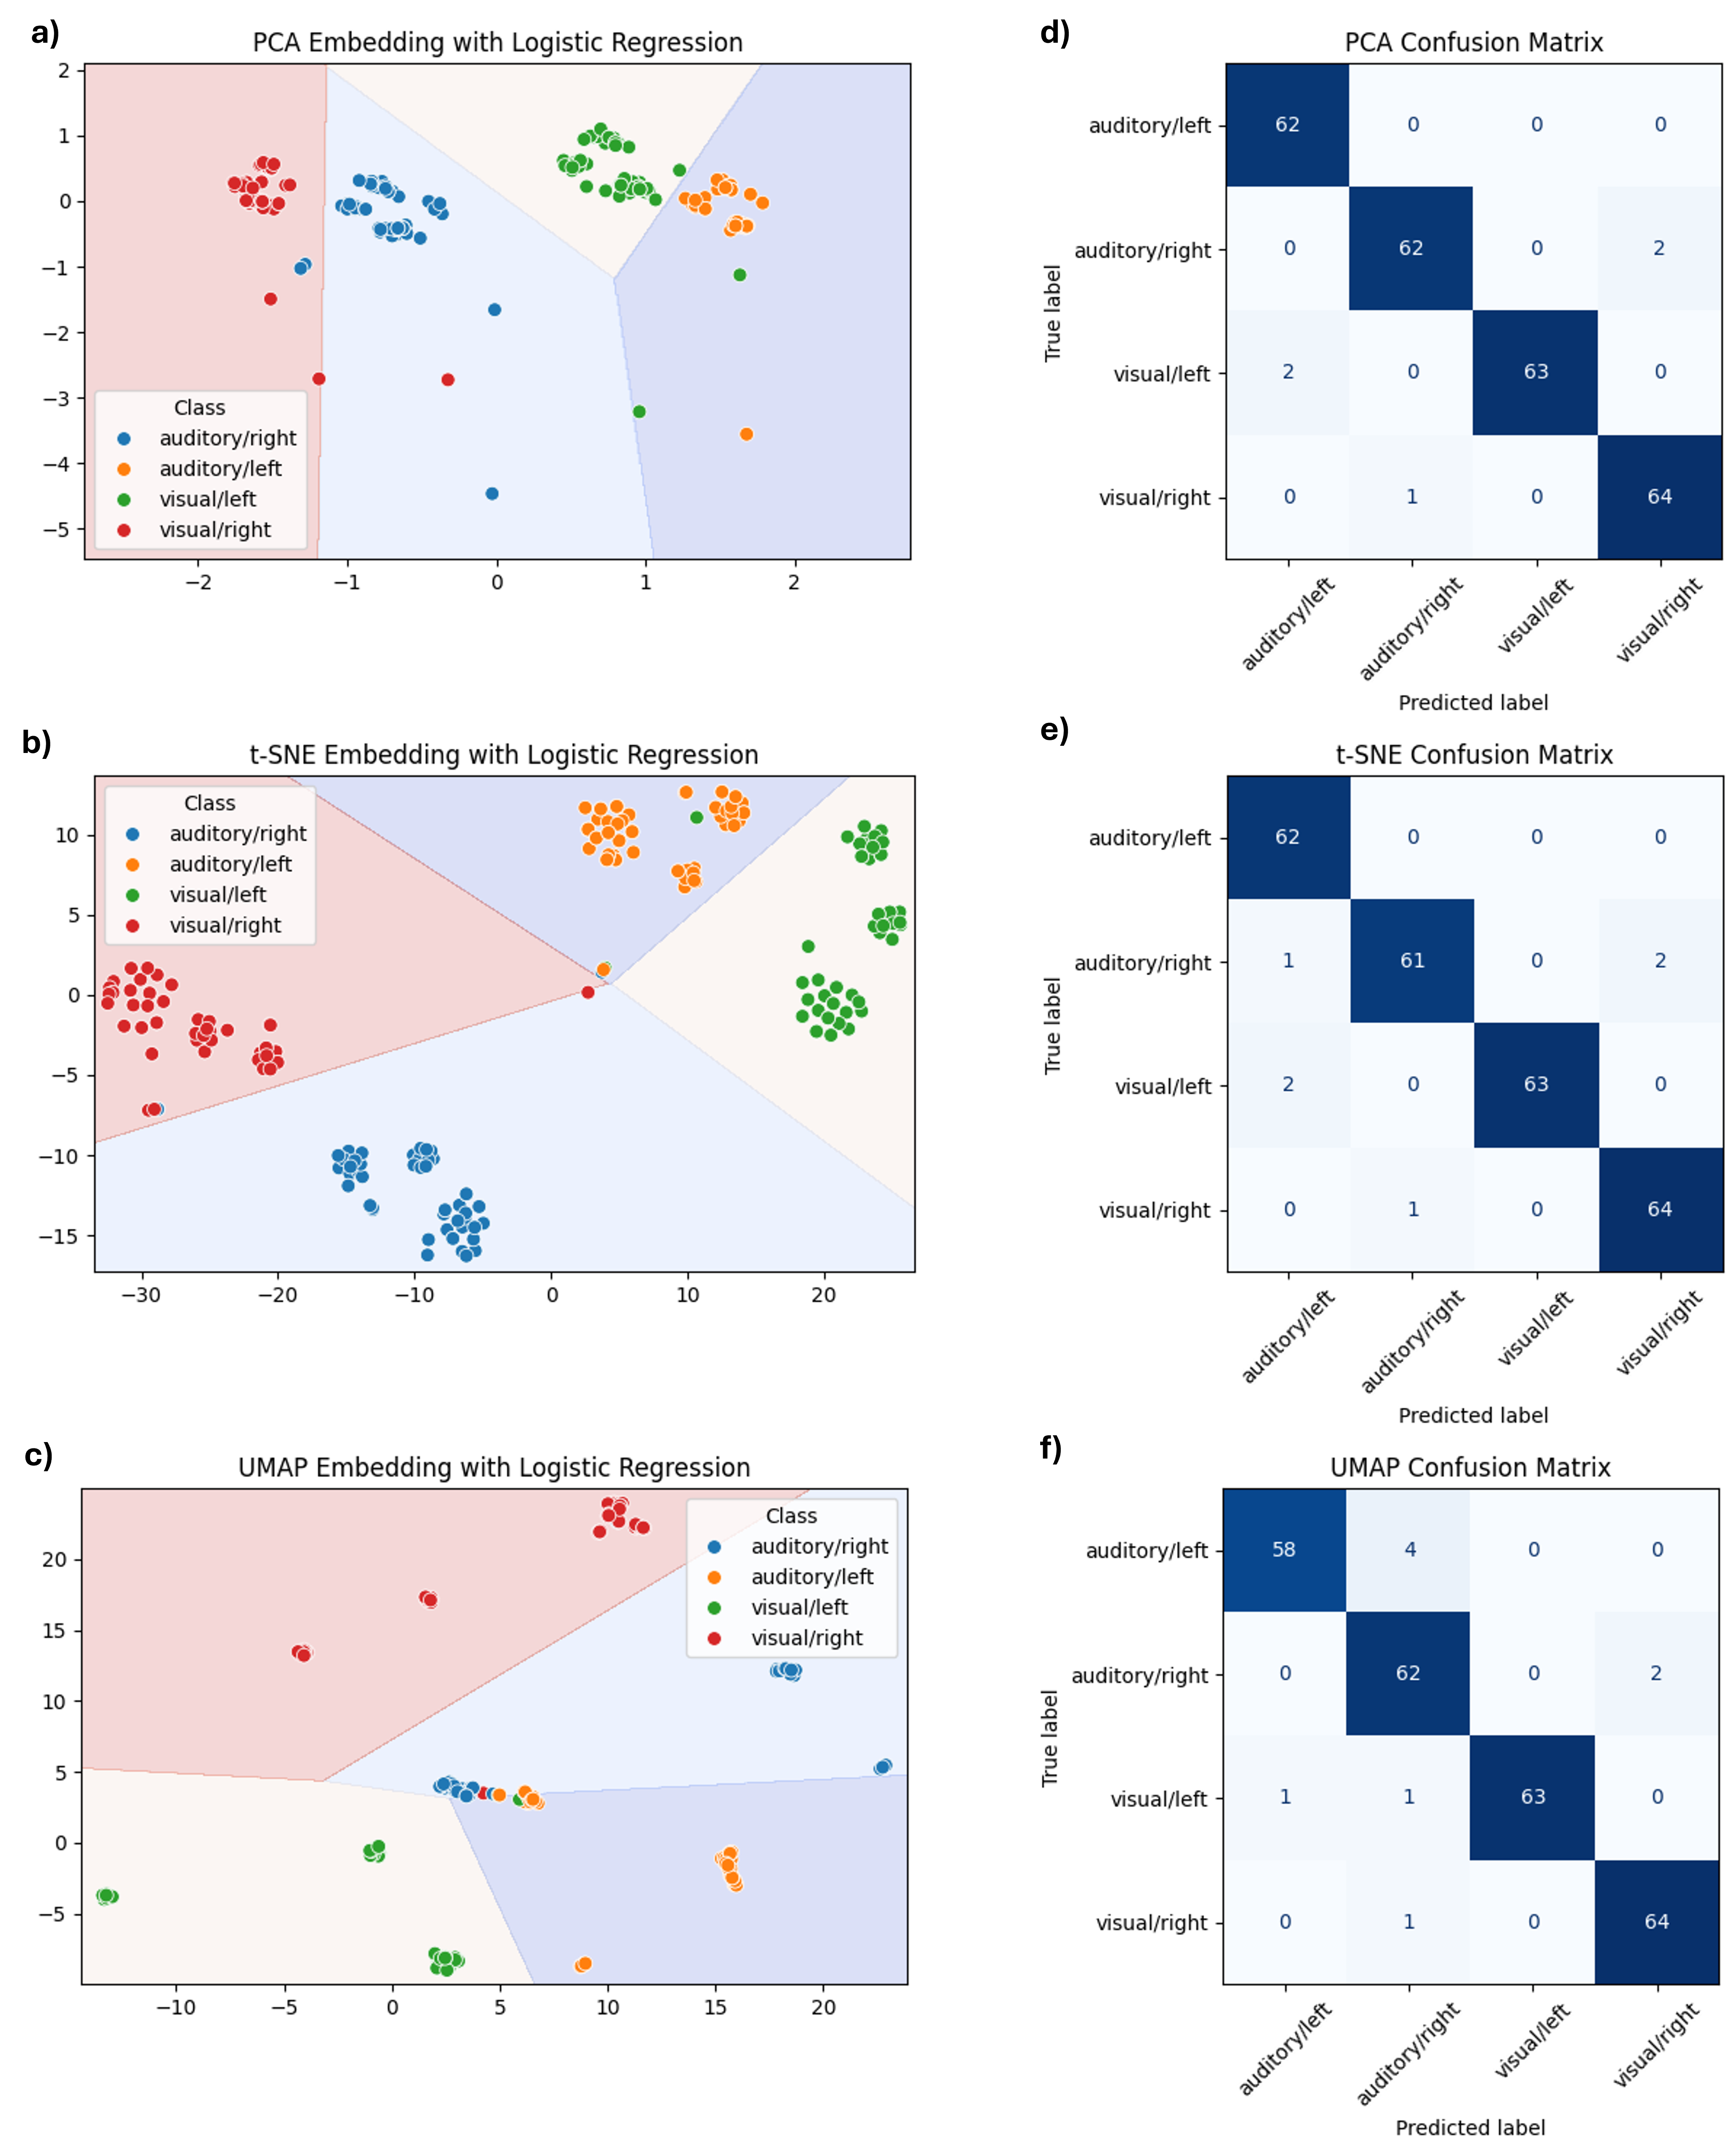
\includegraphics[width=0.95\textwidth]{Chapter7/Figs/f.png}}
    \caption[Visualization of class separability in spiking feature representations using dimensionality reduction techniques.]{Visualization of class separability in spiking feature representations using dimensionality reduction techniques. Each subplot pair displays the output of a trained MCSNN on EEG dataset. Left panel (a-c): 2D embeddings obtained via (PCA / t-SNE / UMAP), colored by ground truth class and overlaid with the decision boundary of a logistic regression classifier.
    Right panel (d-e): Corresponding confusion matrix showing the classifier's performance.}
    \label{fig:7f}
\end{figure}

\noindent Each 2D embedding revealed distinct class separability characteristics. PCA, a linear projection method, produced symmetric decision boundaries with slight overlap between the two auditory classes. This overlap translated to a total of four misclassifications, two for each auditory class, yielding an overall classification accuracy of 97.66\%. In contrast, t-SNE, which preserves local structure through nonlinear manifold learning, achieved the highest separation quality among the three methods. It generated clearly isolated clusters corresponding to each class, resulting in only two misclassifications and an accuracy of 98.44\%. UMAP, which balances local and global structural preservation, also achieved clear cluster formation but displayed some ambiguity at class boundaries, particularly for auditory/left, reducing its accuracy to 96.48\%.
\begin{table}[ht]
    \centering
    \caption{Classification accuracy (\%) for each stimulus class using PCA, t-SNE, and UMAP embeddings followed by logistic regression.}
    \resizebox{\textwidth}{!}{%
    \begin{tabular}{lccccc}
    \toprule
    \textbf{Method} & \textbf{Overall Accuracy} & \textbf{auditory/left} & \textbf{auditory/right} & \textbf{visual/left} & \textbf{visual/right} \\
    \midrule
    PCA  & 97.66 & 96.9 (62/64) & 96.9 (62/64) & 98.4 (63/64) & 100 (64/64) \\
    t-SNE & 98.44 & 98.4 (63/64) & 98.4 (63/64) & 98.4 (63/64) & 100 (64/64) \\
    UMAP & 96.48 & 90.6 (58/64) & 96.9 (62/64) & 98.4 (63/64) & 100 (64/64) \\
    \bottomrule
    \end{tabular}%
    }
    \label{table:7b}
\end{table}

\noindent The confusion matrices in Table \ref{table:7b} further quantify these outcomes. While all methods demonstrated excellent performance on visual/left and visual/right, t-SNE exhibited the fewest misclassifications across all classes. PCA and UMAP both struggled slightly with the auditory classes, particularly auditory/left, which UMAP misclassified six times. These patterns were also visible in the decision boundaries in Figure \ref{fig:7f}, where the UMAP decision region encroached into adjacent auditory clusters.\\

\noindent In addition to classification accuracy, the dimensionality reduction techniques were compared based on their decision boundary characteristics, interpretability, and embedding stability. PCA yielded highly interpretable linear boundaries, although its linearity limited separation in nonlinearly structured data. t-SNE produced highly non-linear, class-specific embeddings with strong cluster compactness, though known to be sensitive to initialization and perplexity. UMAP offered a good compromise between global and local structure, yielding interpretable and stable results, albeit with minor classification degradation due to overlapping auditory representations.\\

\noindent These results demonstrate that low-dimensional embeddings of MCSNN feature maps retain sufficient discriminative power for linear classification. Among the evaluated techniques, t-SNE provided the clearest separation of EEG stimulus categories, reflecting the network's ability to encode modality-specific structure in its spiking representations. Compared to traditional CNN or LSTM models, the proposed memristive CSNN achieves comparable or superior classification performance while eliminating the overhead of recurrent memory modules. \\

\noindent The use of memristor-modeled spiking neurons offers biologically plausible dynamics, compatibility with silicon oxide-based neuromorphic circuits, and reduced power consumption suitable for real-time, edge-deployable EEG systems. This approach demonstrates one of the first successful applications of CSNNs for classifying EEG-based affective or cognitive states without resorting to computationally expensive sequential models.\\

\noindent In the future, SNNs could be adapted as spiking autoencoders, benefiting from their ability to efficiently encode and decode temporal and spatial patterns. This could lead to significant advancements in data compression and anomaly detection. Furthermore, SNNs hold promise in bio-signal processing applications, where their biologically inspired architecture can handle complex signals such as electroencephalograms (EEGs) or electromyograms (EMGs). Future studies should explore these applications, integrating SNNs with biosignal devices or advanced sensors, and enhancing robustness against device non-idealities for real-time biosignal processing.

\section[Summary]{Summary}

\noindent This chapter has explored the design, optimisation, and practical deployment of spiking neural networks (SNNs) using memristive hardware, focusing specifically on the mitigation of device-level non-idealities and the application of these neuromorphic systems to biosignal processing tasks. Beginning with a detailed overview of optimisation challenges unique to analogue memristive circuits, the chapter motivated the necessity for specialised training methods and regularisation techniques that account for the stochastic and constrained nature of physical synapses. \\

\noindent A critical review of existing optimisation algorithms was presented, contrasting early spike-based learning rules such as SpikeProp with more recent surrogate gradient-based approaches. The limitations of current training paradigms were discussed in light of their scalability, computational complexity, and compatibility with temporal data processing. Emphasis was placed on rate-based approximations and function approximation methods as practical alternatives to spike-level learning, especially in larger network architectures. \\

\noindent To address the inherent variability and failure-proneness of memristive devices, the chapter introduced homeostasis-driven dropout regularisation, inspired by biological self-regulatory processes. A novel model was proposed wherein synaptic conductance dynamically decreases with high presynaptic firing rates, thereby suppressing overactive pathways and enhancing the generalisation capacity of the network. Simulation results demonstrated the effectiveness of this mechanism across both fully connected and convolutional SNN architectures, with accuracy improvements exceeding 20\% in the presence of up to 50\% device failure.\\

\noindent The chapter then extended its scope to the application of memristive SNNs in biosignal classification, particularly focusing on electroencephalogram (EEG) data. A hybrid Convolutional Spiking Neural Network (CSNN) architecture was designed, integrating spatial convolutional filters with Leaky Integrate-and-Fire dynamics to process temporally encoded spike trains. The model was evaluated on real EEG data acquired from simultaneous MEG/EEG experiments, with preprocessing and spike encoding methods tailored for temporal fidelity and biological plausibility.\\

\noindent Quantitative evaluation of the trained model using dimensionality reduction techniques such as PCA, t-SNE, and UMAP revealed robust class separability and high classification accuracy (up to 98.44\%), demonstrating the capability of memristive CSNNs to extract meaningful spatiotemporal features from complex biological signals. The UMAP-based projections offered a balance between global and local data structure, while t-SNE achieved the highest discriminative performance across stimulus categories. \\

\noindent Collectively, this chapter demonstrates that memristive SNNs—when augmented with biologically inspired learning mechanisms and probabilistic models of hardware imperfections—can serve as resilient, energy-efficient alternatives to conventional neural networks. Their integration with dropout-based homeostasis, convolutional structures, and neuromorphic encoding strategies makes them particularly well-suited for real-time, edge-deployable applications in cognitive monitoring, brain-computer interfacing, and neuromorphic signal processing. These findings contribute a foundational framework for future exploration of large-scale, hardware-constrained spiking systems in dynamic, sensor-rich environments.\\